\chapter{Discussion}

% Start with the big picture.
Our analysis of the Orion A and Orion B molecular clouds reveals a complex interplay between morphology, topology, and star formation activity. 
By combining perimeter–area scaling, Euler characteristic profiles, and mass–size relations, we obtain a consistent picture of how structural complexity varies across column densities and how these variations relate to the presence of young stellar objects.

% Synthesize the fractal dimension results (global and local).
% To-Do:
% Visuals
The global fractal dimension is based on the idea that if a structure is self‑similar—i.e., lacks a characteristic scale—its perimeter and area should follow a power‑law scaling, appearing as a straight line in a log–log diagram.  
Turbulence is known to play a key role in organizing structure within molecular clouds, and the perimeter–area method provides a way to quantify how much this self‑similar behavior influences the observed morphology.

Our global perimeter–area analysis reveals distinct structural regimes within Orion~A, with a clear change in slope that reflects different levels of complexity at low and high column densities.  
In contrast, Orion~B maintains a more uniform fractal signature.  
This contrast already begins to suggest that Orion~A and Orion~B are governed by different physical conditions.

For Orion~A, a double fit is required, indicating a change in the underlying physics.  
This transition occurs at a column density of \(N = 1.23 \times 10^{22}\,\mathrm{cm}^{-2}\), marking a physically significant scale.  
At this threshold, the structural properties of Orion~A shift, coinciding with the onset of active star formation and the emergence of dense cores \cite{lada2010star}.  
The concurrent changes in fractal dimension and topology at this scale suggest a direct link between the cloud’s morphology and the physical processes driving star formation.

Without applying the double fit, the global fractal dimension is \(D = 1.35 \pm 0.01\).  
This value is in good agreement with previously reported fractal dimensions for molecular clouds derived with alternative methods \cite{elmegreen1996fractal}, where typical values are around \(D \sim 1.3\).  
Numerical simulations based on two‑dimensional compressible turbulence in a self‑gravitating ISM also reproduce similar values \cite{1994fns..book..515Y}.  
Note that many studies report the three‑dimensional fractal dimension, which is related to the two‑dimensional value by adding unity.

When the data are separated into two regimes, we obtain \(D = 1.65 \pm 0.01\) at higher column densities and \(D = 0.97 \pm 0.03\) at lower column densities.  
Although a fractal dimension smaller than 1 is not expected in theory, this result is likely influenced by the limited number of data points contributing to the low‑density fit.  
Even so, the trend is informative: a fractal dimension approaching 1 indicates smoother, simpler boundaries, whereas higher column densities exhibit more complex, space‑filling structures.

% do we see this visually?
With these types of methods, it is important to also consider if our conclusion match what we actually see in the cloud. To this end, we see in the Gallery that: 

Taken together, these results suggest that the processes driving self‑similarity—such as turbulence—become less dominant once dense cores emerge.  
Beyond this threshold, the cloud’s structure deviates from scale‑free behavior, reflecting the impact of star formation on its morphology.

In Orion~B, by contrast, no such break is required.  
This outcome is broadly consistent with expectations, as Orion~B is known to be a more turbulent molecular cloud.  
In such an environment, scale‑free behavior dominates across the column‑density range analyzed, as reflected in the high quality of the single global fractal dimension fit.  
The emergence of cores does not appear to disrupt the hierarchical structuring.  
Together, these findings provide the first elements of a coherent picture described by the Minkowski functionals.

% do we see this visually?
Again, we need to ask ourselves if visually these conclusions make sense.

It is also instructive to compare these results with measurements obtained for other molecular clouds.  
Studies applying perimeter–area methods or similar techniques have typically found global fractal dimensions in the range \(D \sim 1.2{-}1.4\) for nearby star‑forming regions.  
For example, \cite{falgarone1991hierarchical} reported \(D \approx 1.36\) for CO maps of Perseus and Ophiuchus, while \cite{sanchez2005fractal} found values between 1.25 and 1.35 for a sample of Galactic molecular clouds.  
These values are broadly consistent with the single‑fit results for Orion~A (\(D = 1.35 \pm 0.01\)) and Orion~B (\(D = 1.40 \pm 0.01\)), reinforcing the interpretation that the large‑scale morphology of these clouds is comparable to that of other regions in the Milky Way.

What is less commonly reported, however, is the clear break we observe in Orion~A at \(N = 1.23 \times 10^{22}\,\mathrm{cm}^{-2}\).

Naturally, this method has limitations.  
Numerical errors can arise when calculating perimeters and areas for very small structures at high column densities.  
Straight contours, resulting from limited observational resolution, should also be avoided, as they can distort the scaling relationships on which the method relies.

The local fractal dimension takes instead the base of the perimeter-area relation and inverse it to obtain a proxy for the complexity of single structures.
This picture is a bit more complex, but more faceted as well. 

The local fractal dimension, calculated at each column density threshold shows a remarkable trend towards 2 at higher column density threshold for both Orion A and B. This seems to be caused not by the complexity of the single structures, but rather by the sprawling network of cores, fibers and filaments that appear as the structure breaks down at higher column densities.

% do we see this visually?
Some visual examples are also useful to picture this: see Gallery. The peaks can represent:

The method has some limitations, as straight lines and low resolution data (at low-column densities) and structures that are too small (at high column densities) can affect the results, and hence why the column density range is not as extended as the maps can actually offer.

% Integrate topological insights (Euler characteristic).
% To-Do:
% Remake Images (after making sure that the definition is correct)
Furthermore, the Euler characteristic highlights clear differences between Orion~A and Orion~B.  
Orion~A exhibits a profile that closely resembles the behavior expected from Gaussian Random Field simulations, with a well-defined peak at approximately \(1.64 \times 10^{22}\,\mathrm{cm}^{-2}\).  
This threshold is significant, echoing the transition seen in the global fractal dimension analysis, and marks the emergence of dense cores within the cloud.

In contrast, Orion~B shows no such pronounced peak, instead displaying a more gradual, almost linear decrease.  
If Orion~B is indeed more strongly influenced by turbulence, this behavior is consistent with a more scale-free, less clustered structure, where the appearance of dense cores is more gradual and widely distributed.  
The topological analysis therefore reinforces the notion that turbulence governs the structural evolution of Orion~B, while Orion~A undergoes distinct transitions closely tied to star-formation thresholds.

Visual examples of the changes in the Euler characteristic for Orion~A and Orion~B are provided in Figures~\ref{fig:Euler_Orion_A} and~\ref{fig:Euler_Orion_B}.

\begin{figure}[t]
    \centering
    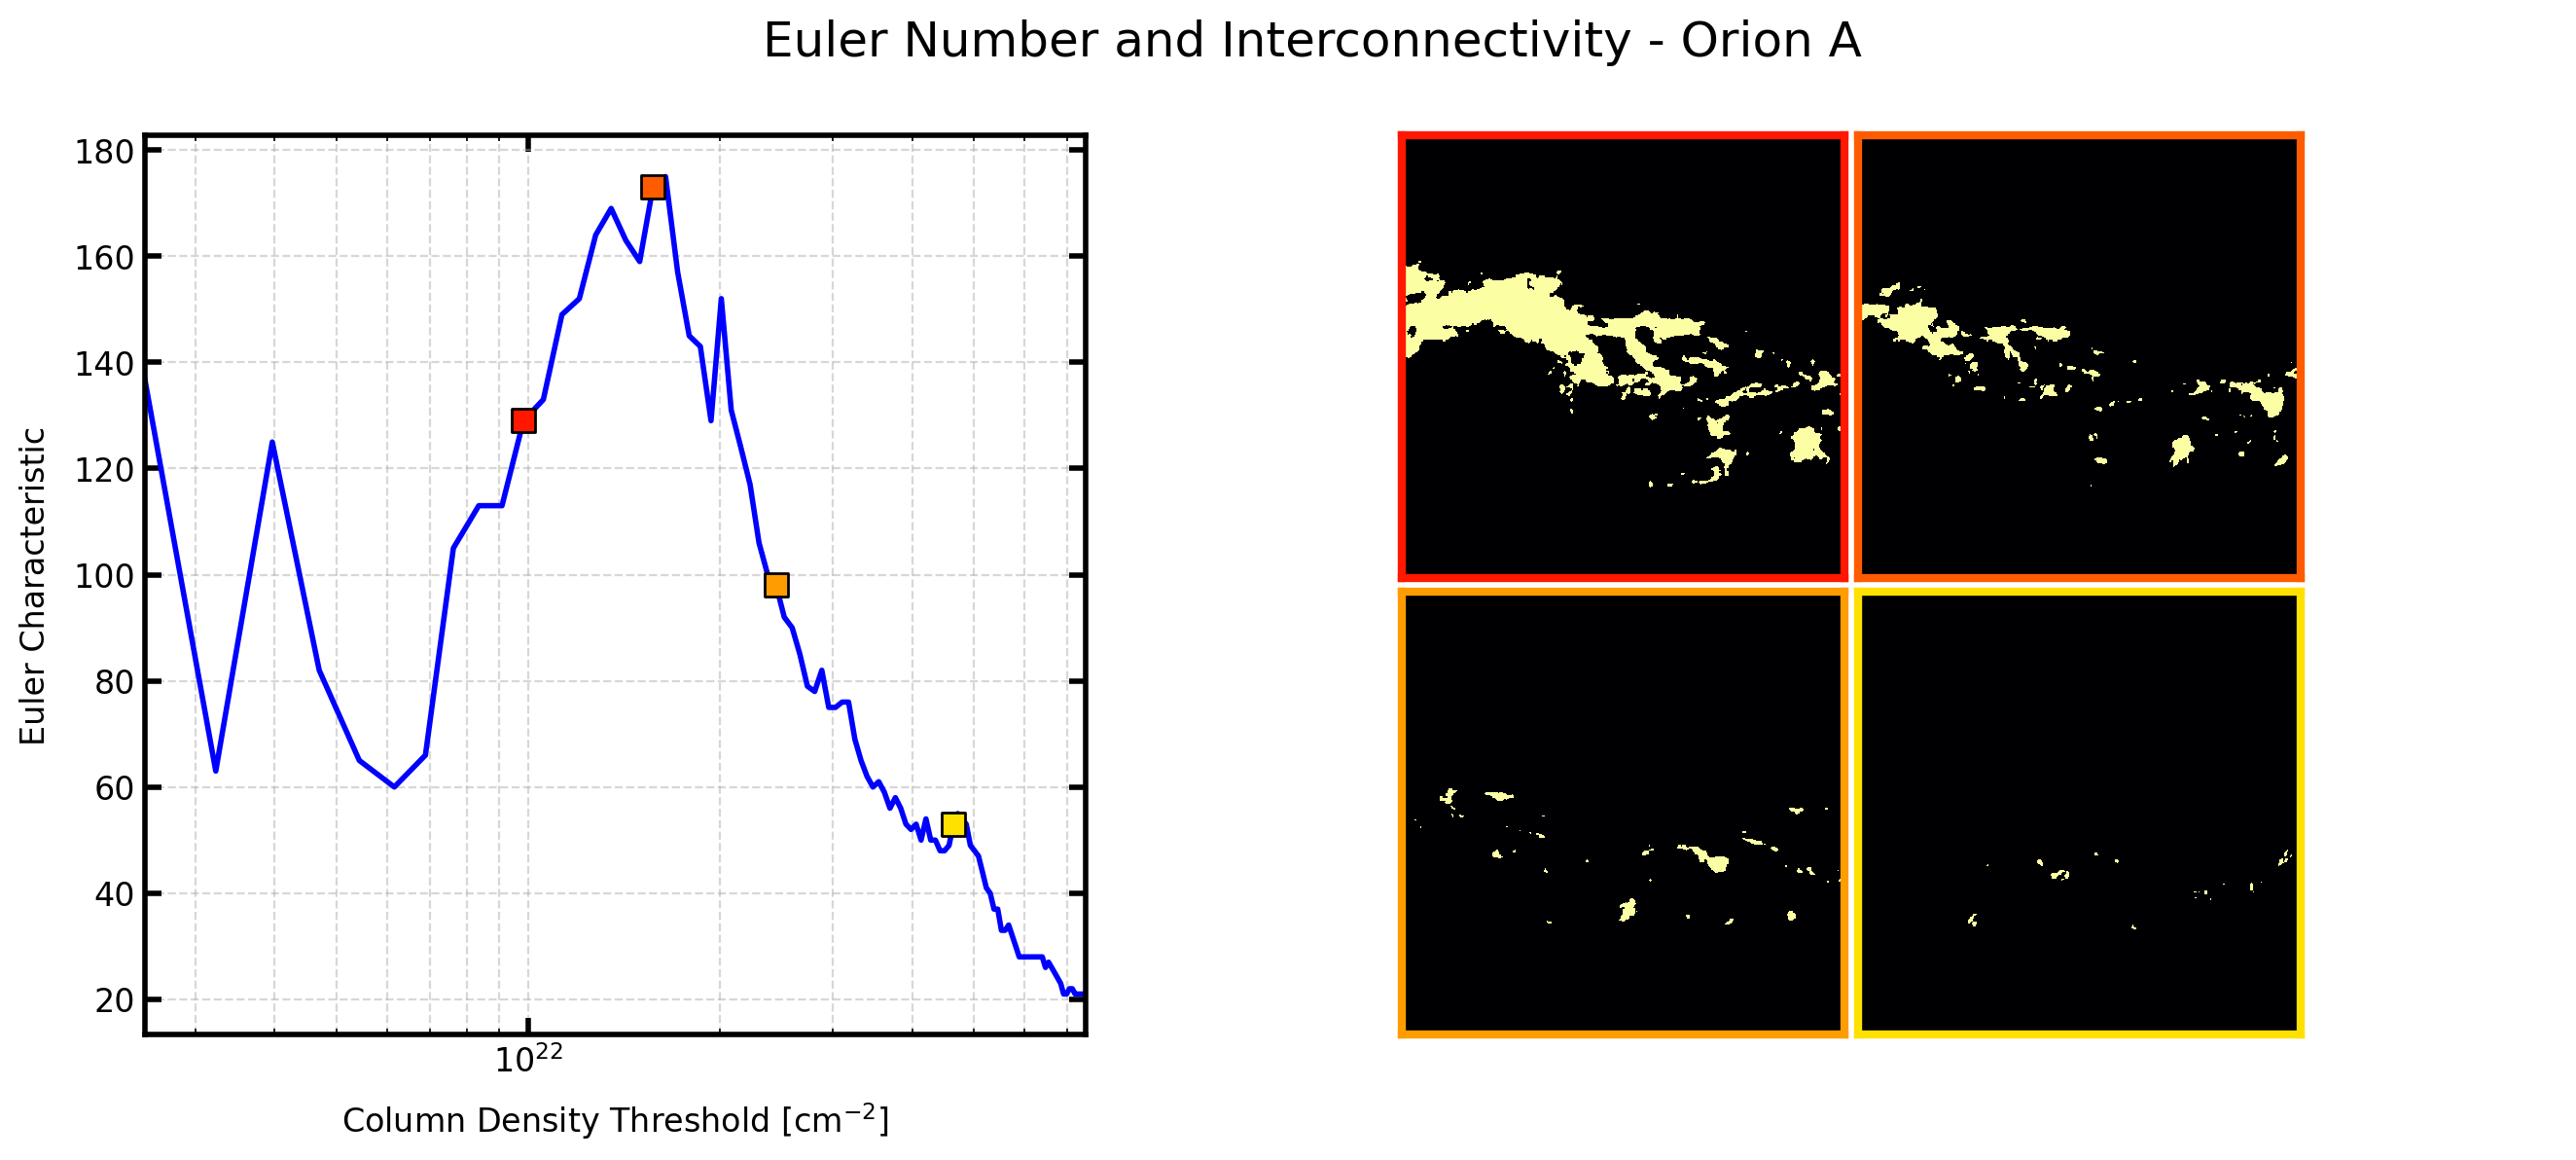
\includegraphics[width=0.65\textwidth]{figures/euler_Orion_A.png}
    \caption{Euler characteristic as a function of column density (left) and four examples of structures (right) marked by colored boxes on the graph (Orion A).}
    \label{fig:Euler_Orion_A}
\end{figure}

\begin{figure}[t]
    \centering
    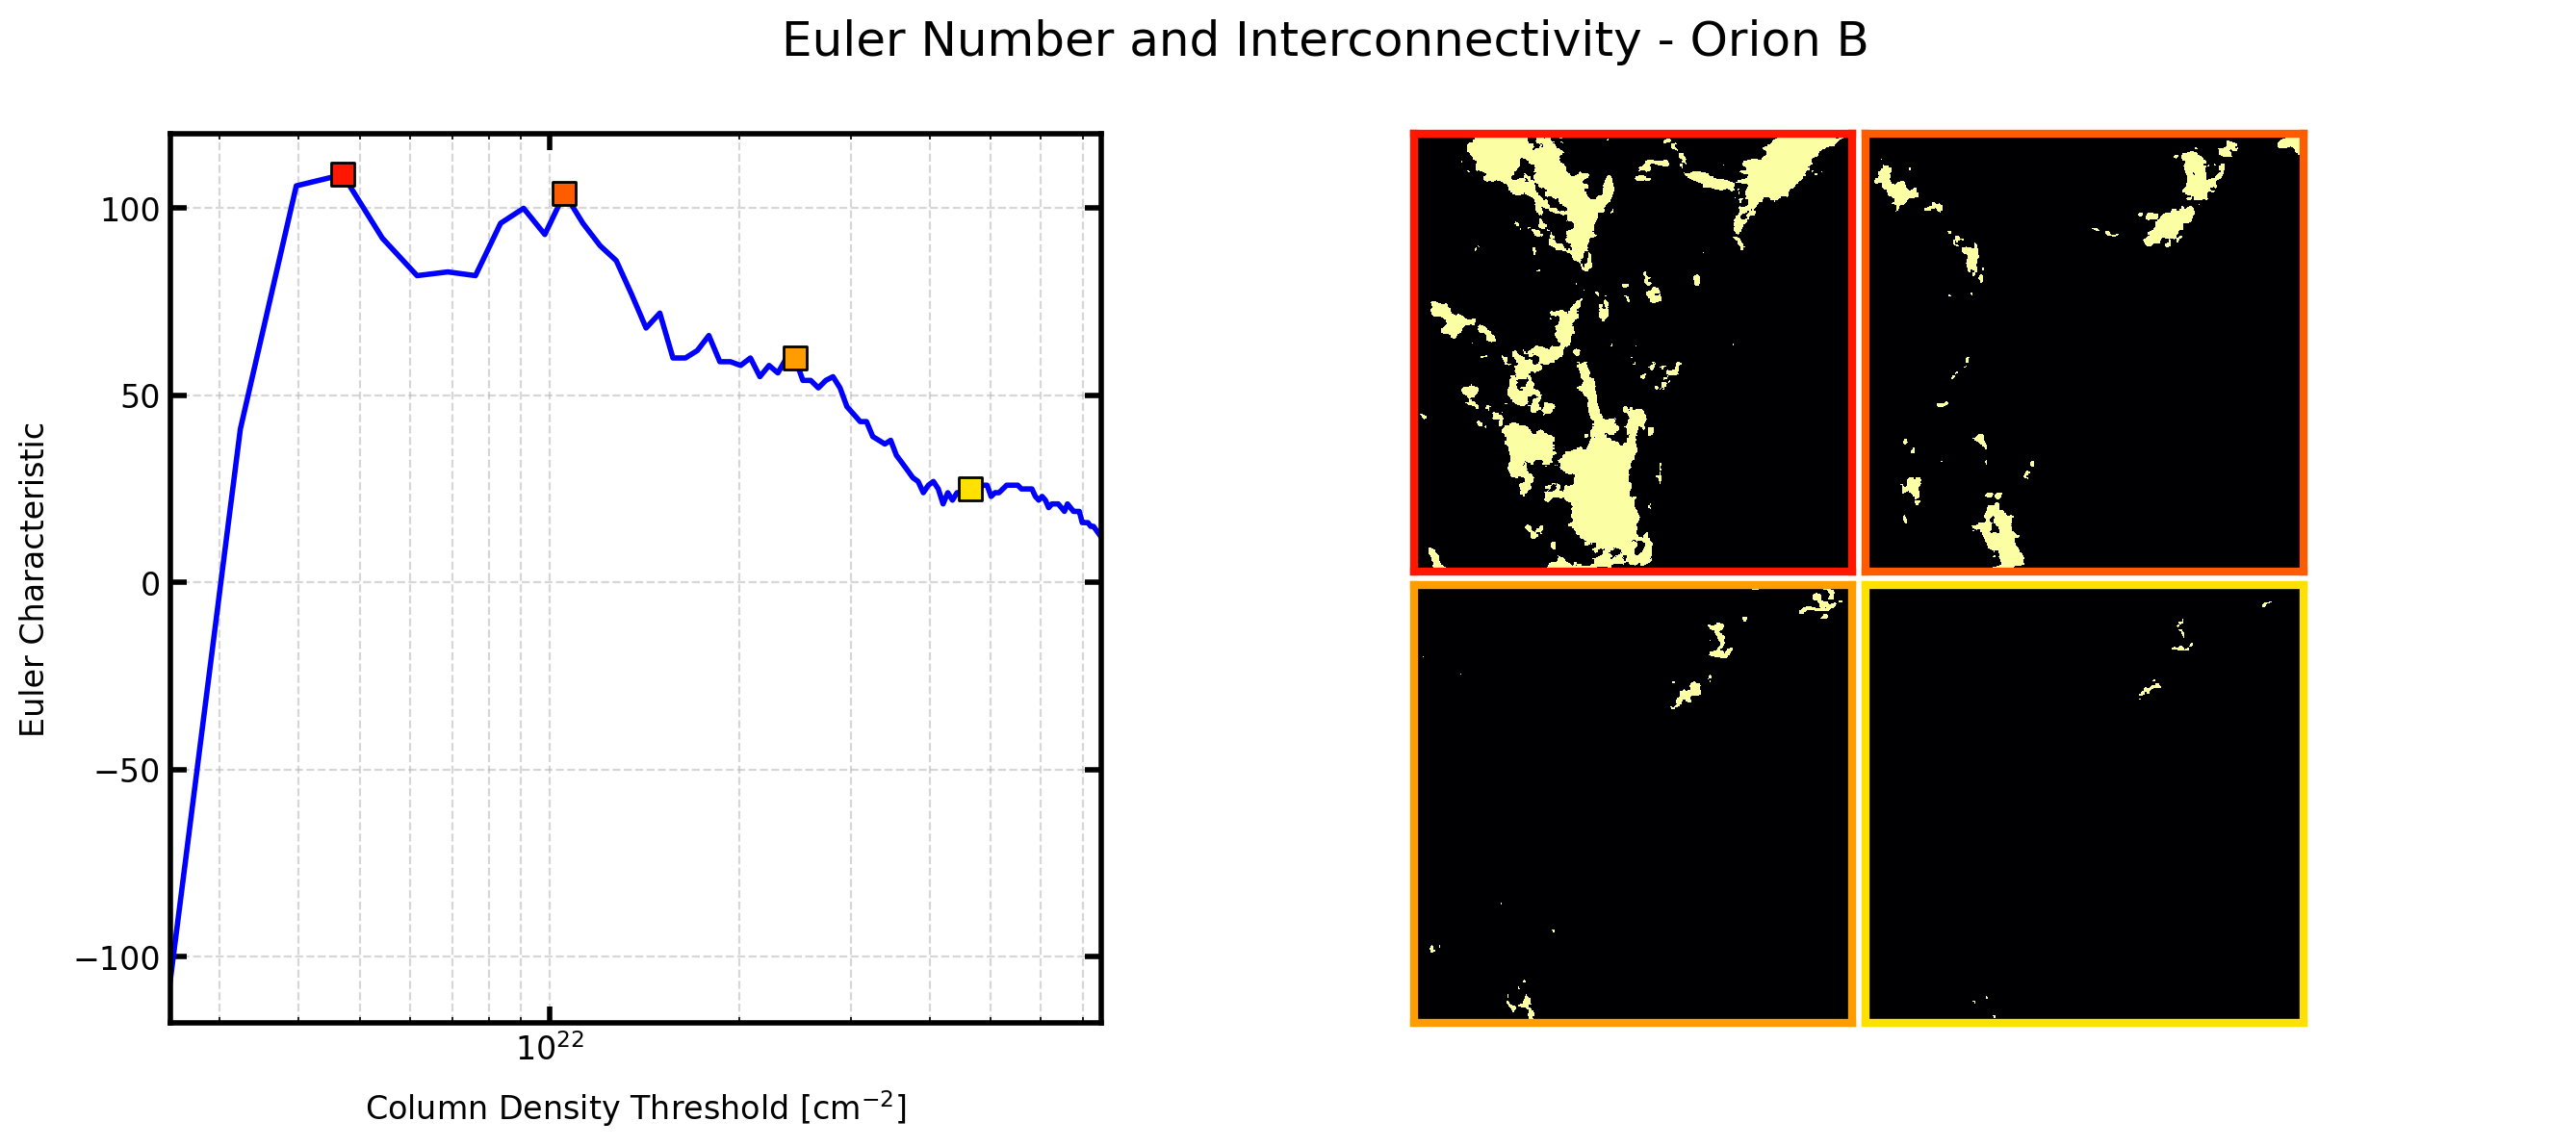
\includegraphics[width=0.65\textwidth]{figures/euler_Orion_B.png}
    \caption{Euler characteristic as a function of column density (left) and four examples of structures (right) marked by colored boxes on the graph (Orion B).}
    \label{fig:Euler_Orion_B}
\end{figure}

% Bring in the MSD plane and individual-structure analysis.

% Connect to star formation.
% which of the two is forming more stars?

% End with a synthesis.


% Global Fractal Dimension 
% Orion B is more turbulent and we can defo see that 
% Orion A double fit -> the changing point is where stars from
% We see that point also in the Euler Characteristic
% Less so in Orion B, this gives a coherent picture of how the Minkowski functionals can describe the physics of the cloud.
% Reference that one paper for the local fractal dimension

comparison with the M**alpha method

Star Formation: method a bit limited by the number and extent of the objects.